\section{Related Work}

Previous work applying augmented reality to retail shopping has focused on how designers and system architects properly utilize this novel technology. Ahn et al. employed augmented reality to promote health-oriented shopping \cite{ahn2015supporting}, and similarly, Cenieros et al. focused on environmentally-conscious shopping \cite{ceniceros2014augmented}. These and other works \cite{esser2016head,stoyanova2015comparison} discuss the influence augmented reality can have in a store environment. Context-awareness is a useful affordance provided by augmented reality.  Designers find that this ability to visually associate digital content with products increases customer empowerment, user efficiency in gathering information, and system influence \cite{kourouthanassis2007enhancing,olsson2013expected,zhu2004personalized}. Augmented reality application work has additionally focused on collaborative experiences and visualizations \cite{esser2016head,santos2016augmented,stoyanova2015comparison,truong2013today}. These efforts highlight the importance of context-awareness and visualization provided by augmented reality in providing new functionality. However, we engage in a user-centered design process to identify aspects of existing parallel experiences in order to merge those experiences to one that is useful and familiar.

\begin{marginfigure}
	\begin{minipage}{\marginparwidth}
		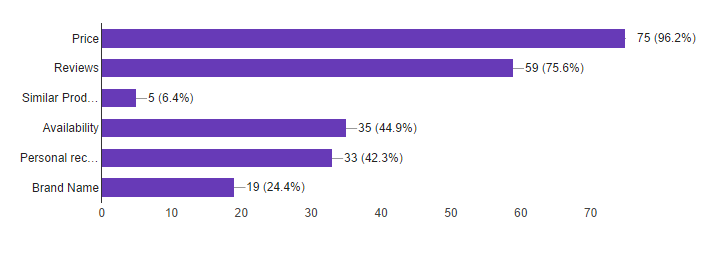
\includegraphics[width=0.9\columnwidth]{figures/ShoppingFactors}
		\caption{Phase One respondants identified price and reviews as the most critical factors in making their shopping decisions, while product comparisons---identified in later phases as ``highly useful''---were initially rated as least important.}
		\label{figures:ShoppingFactors}
	\end{minipage}
\end{marginfigure}

Much of this previous work has focused on mobile augmented reality (MAR). However, MAR systems suffer from a number of limitations for retail shopping such as insufficient processing power, required use of hands and an intermediate screen, and a field of view constrained by screen size \cite{bimber2005spatial}. Head-mounted displays (HMDs) such as Microsoft's Hololens offer opportunities to overcome these limitations, and the ability to synchronize data with head movements may allow consumers passive access to visual information in context. In this work, we explore how systems might effectively leverage HMDs to provide product information in context for traditional retail environments. 

%MW: Removed for space.
%Other work has introduced spatial augmented reality (SAR) systems and applications.  SAR applications employ ubiquitous computing to project context-aware digital content into the user's physical environment \cite{benko2015fovear,benko2014dyadic}.  Technical advantages of a SAR system include removing the need for users to wear or carry often cumbersome equipment and a non-restricted field of view.  \todo{DNS: yep, really might be good to blend with the previous paragraph and leave some space to talk about design since that is a contribution of the work} However, one limitation of SAR systems is that they require a static, controlled environment to be used effectively due to the use of fixed displays \cite{bimber2005spatial}.

In this paper, we take a user-centered design approach to testing how the grounding of design principles derived from this previous work on mobile augmented reality applies to HMD-based augmented reality. We also examine how HMD-based AR may combine some of the benefits of these approaches while removing some of their limitations. Our work iterates on this approach in three distinct development phases: an open-ended survey, a low fidelity prototype, and a high fidelity prototype.